\documentclass{article}
\usepackage{tikz,tcolorbox}
\usepackage{array} % For customizing tables
\usepackage{booktabs} % For better horizontal lines
\usepackage[a4paper, paperwidth=25cm, paperheight=25.5cm, left=2cm, right=2cm, top=2cm, bottom=2cm]{geometry}
\usepackage{multicol}
\usepackage{amsmath}
\usepackage{pgfplots}
\usepackage{makecell}
\usetikzlibrary{patterns}
\definecolor{greenPlot}{HTML}{14C877}
\definecolor{orangePlot}{HTML}{EA6E12}
\definecolor{purplePlot}{HTML}{4C12EA}
\definecolor{blueArea}{HTML}{10D9EE}
\definecolor{redPlot}{HTML}{ED014A}
\definecolor{box}{HTML}{27C1A0}
\definecolor{pur}{HTML}{A128E1}

\tcbuselibrary{skins, breakable, theorems}

\newtcolorbox{prettyBox}[2]{
  enhanced,
  colback=white!90!#2,   % Background color based on the second parameter (color)
  colframe=#2!60!black,  % Frame color based on the second parameter (color)
  coltitle=white,        % Title color (white)
  fonttitle=\bfseries\Large,
  title=#1,              % Title from the first parameter
  boxrule=1mm,
  arc=0.5mm,
  drop shadow=#2!35!gray, % Drop shadow color based on the second parameter (color)
}




\setlength{\parindent}{0pt}
\setcellgapes{3pt}  % Adjust padding as needed
\makegapedcells
\begin{document}
\renewcommand{\arrayrulewidth}{0.75mm} % Set line thickness
\setlength{\tabcolsep}{12pt} % Set horizontal padding
\renewcommand{\arraystretch}{1.5} % Set vertical padding (1.0 is default)
\section{What's Operations Research?}
\begin{tcolorbox}[title=Definition]
Operations Research (\textbf{OR}) is an interdisciplinary field that uses mathematical models, statistical analysis, 
and optimization techniques to help solve complex decision-making problems and achieve the most efficient outcomes.
\noindent it involves the use of several key techniques, including:

\begin{itemize}
    \item \textbf{\underline{Optimization}}: Finding the best solution based on given criteria.
    \item \textbf{\underline{Mathematical Modeling}}: Representing real-world scenarios through mathematical equations and models.
    \item \textbf{\underline{Statistical Analysis}}: Using data to analyze and predict outcomes.
    \item \textbf{\underline{Simulation}}: Testing strategies in a controlled model environment.
\end{itemize}
The goal of Operations Research is to offer data-driven insights and methods that lead to more informed, optimized decisions.
\end{tcolorbox}

\section{Origin of Operations Research}

\begin{tcolorbox}[title=Origin]
Operations Research (\textbf{OR}) originated during World War II, when the British government assembled a team of analysts, 
scientists, engineers, and military officers to study complex operational problems such as : air defense, bombing strategies, 
convoy routing, and other crucial military operations . Using mathematical models and data analysis, the team simulated various scenarios 
to predict outcomes and recommend optimal decisions. The success of these methods in improving military strategy inspired 
other nations to adopt similar approaches.This eventually led to the formalization of OR as a scientific discipline after the war.
\end{tcolorbox}

\section{Types of Problems Treated by OR}

\begin{tcolorbox}[title=Types of Problems]
Operations Research (\textbf{OR}) focuses on solving real-world problems by finding the most optimal decisions.The types of problems OR addresses can generally be categorized as:

\begin{itemize}
    \item \textbf{\underline{Maximization}}: Achieving the highest possible value for an objective, such as maximizing profits, productivity, or efficiency. 
        \begin{itemize}
            \item Example: Maximizing a company's revenue by determining the most profitable product mix.
        \end{itemize}
    
    \item \textbf{\underline{Minimization}}: Reducing or minimizing undesirable factors, such as costs, time, or resource consumption.
        \begin{itemize}
            \item Example: Minimizing the cost of materials in manufacturing while maintaining quality standards.
        \end{itemize}

    \item \textbf{\underline{Optimization}}: Finding the best possible solution from multiple alternatives, often involving both maximization and minimization aspects. 
        \begin{itemize}
            \item Example: Finding the shortest path in a transportation network or optimizing team roles in a project.
        \end{itemize}
\end{itemize}
\end{tcolorbox}

\section{Algorithm Complexity}

\begin{tcolorbox}[title=Algorithm Complexity]
Algorithm complexity refers to the amount of computational resources an algorithm uses. These resources are typically categorized as:

\begin{itemize}
    \item \textbf{Time Complexity}: The amount of time it takes for an algorithm to run, depending on the size of the input.
    It is commonly expressed using Big O notation (e.g., \(O(n)\), \(O(\log n)\)), which describes the algorithm's growth rate
    as the input size increases.
    
    \item \textbf{Space Complexity}: The amount of memory or space an algorithm requires. This is influenced by the number and 
    size of variables, data structures, and other memory-using elements.
\end{itemize}

Minimizing both time and space complexity is crucial when developing efficient algorithms, as it leads to more optimal performance, especially for large-scale problems.
\end{tcolorbox}


\section{Linear Programming}
\subsection{What's Linear Programming ?}
\begin{tcolorbox}[title = Definition] 
    tcolorbox
\end{tcolorbox}
\vspace{1cm}
\begin{center}
    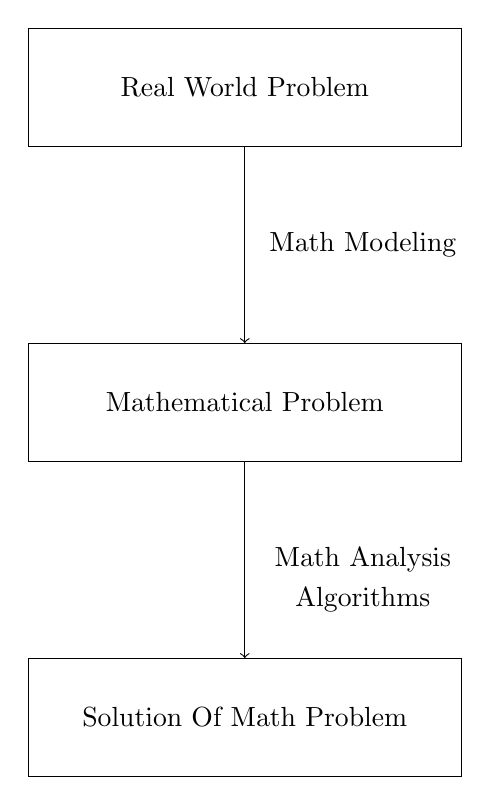
\begin{tikzpicture}
       \draw (0,0) rectangle (5.5,1.5);
       \node at (2.75,0.75) {Real World Problem};
      
       \draw[->] (2.75,0) -- (2.75,-2.5);
       \node at (4.25,-1.25) {Math Modeling};

       \draw (0,-4) rectangle (5.5,-2.5);
       \node at (2.75,-3.25) {Mathematical Problem};
      
       \draw[->] (2.75,-4) -- (2.75,-6.5);
       \node at (4.25,-5.25) {Math Analysis};
       \node at (4.25,-5.75) {Algorithms};
       
       \draw (0,-8) rectangle (5.5,-6.5);
       \node at (2.75,-7.25) {Solution Of Math Problem};
   \end{tikzpicture}
\end{center}
\vspace{1cm}
\subsection{Modeling}
\textbf{\large{\underline{Example :} Diet Problem}}\\

\vspace{0.25cm}
The Goal is to minimize food cost but to meet the minimum daily nutrition requirement
\vspace{1cm}
\begin{center}
\begin{tabular}{|c|c|c|c|c|c|}
    \hline
    Food & Units & Protein & Vit c & Iron & Price\\
    \hline
    Apples & 1 med & 0.4 & 6 & 0.4 & 8\\
    \hline
    Banana & 1 med & 1.2 & 10 & 0.6 & 10\\
    \hline
\end{tabular}
\end{center}

\vspace{1cm}

\begin{multicols}{2}
\textbf{\underline{Variables Definition:}}\\

Let \(x_1\) be the number of Daily Unit Appels.\\

Let \(x_2\) be the number of Daily Unit Banana.\\
\columnbreak

\textbf{\underline{Constraint:}} 

\[
\left\{
    \begin{array}{l}
        \forall x_1 , x_2 \geq 0 \quad \text{(Non-negative number of food item) ...C1}\\\\
        0.4x_1 + 1.2x_2  \geq 70 \quad \text{(Minimum Protein Daily) ...C2}\\\\ 
        6x_1 + 10x_2  \geq 50 \quad \text{(Minimum Vitamine c Daily) ...C3}\\\\
        0.4x_1 + 0.6x_2  \geq 12 \quad \text{(Minimum Iron Daily) ...C4}
   \end{array}
   \right.
\] 
\end{multicols}
\vspace{0.5cm}
\begin{tcolorbox}[title = Objectif Function]
\[
f(x) = 8x_1 + 10x_2  
\]
\begin{center}
The goal is to minimize food cost by maximizing \(f(x)\), while meeting the minimum daily nutrition .
\end{center}
\end{tcolorbox}
\vspace{1cm} 
\textbf{\underline{Problem :}} Find the minimum of \(f(x_1,x_2) \) subject to the contraints\\
\subsection{Graph Model}
This model is used when the objective fucntion has 2 variables consist into turning all the constraint into 
lines and then finding the feasible region and then to search for min or max of the objective function 

\vspace{1cm}
\textbf{Feasible Region :}

\vspace{1cm}
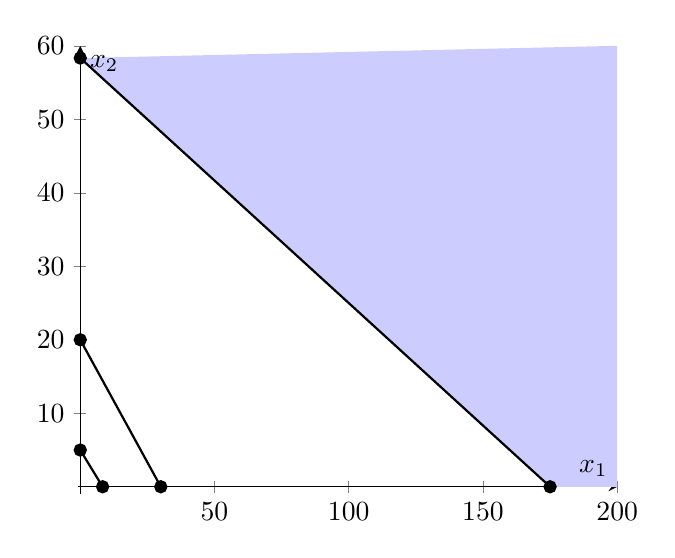
\begin{tikzpicture}
    \begin{axis}[
        axis lines = middle,           % Ensures axes cross at (0, 0)
        xlabel=$x_1$, 
        ylabel=$x_2$, 
        xmin = -1, xmax = 200,           % Set x-axis range
        ymin = -1, ymax = 60,           % Set y-axis range
       ytick={0,10,...,70},             % Y-tick values
        xtick={0,50,...,200},
    ]
  \addplot [draw=none, fill=blue!20] coordinates {(175,0) (200,0) (200,60) (0,70/1.2)}; 
  \addplot[thick, mark=*] coordinates {(175,0) (0,70/1.2)}; 
  \addplot[thick, mark=*] coordinates {(50/6,0) (0,5)};
  \addplot[thick, mark=*] coordinates {(30,0) (0,20)};
\end{axis}

\end{tikzpicture}

\end{document}
